\documentclass{beamer}
\usepackage[T1]{fontenc}
\usepackage[utf8]{inputenc}
\usepackage[german]{babel}
\usepackage{graphicx}
\usepackage{subcaption}
\usepackage{bytefield}
\usepackage{mathtools}
\usepackage[all]{xy}

\usetheme{Warsaw}

\setbeamercolor{normal text}{fg=white,bg=black!90}
\setbeamercolor{structure}{fg=white}

\setbeamercolor{alerted text}{fg=red!85!black}

\setbeamercolor{item projected}{use=item,fg=black,bg=item.fg!35}

\setbeamercolor*{palette primary}{use=structure,fg=structure.fg}
\setbeamercolor*{palette secondary}{use=structure,fg=structure.fg!95!black}
\setbeamercolor*{palette tertiary}{use=structure,fg=structure.fg!90!black}
\setbeamercolor*{palette quaternary}{use=structure,fg=structure.fg!95!black,bg=black!80}

\setbeamercolor*{framesubtitle}{fg=white}

\setbeamercolor*{block title}{parent=structure,bg=black!60}
\setbeamercolor*{block body}{fg=black,bg=black!10}
\setbeamercolor*{block title alerted}{parent=alerted text,bg=black!15}
\setbeamercolor*{block title example}{parent=example text,bg=black!15}


\title{GPUDirect MPI Communications and Optimizations to Accelerate FFTs on Exascale Systems}
\subtitle{Seminararbeit im Masterstudium an der OTH Regensburg}
\author{Robert Graf, Tobias Seitz}

\begin{document}
\frame
{
	\titlepage
}

\frame
{
	\frametitle{Beispieltitel}
	BlaBlaBlubberBlubberFaselBlabla
	\begin{itemize}
		\item Erstens
		\item Zweitens
		\item Drittens
		\item etc.
	\end{itemize}
}

\frame
{
	\begin{center}
		\Large Kommunikationskostenoptimierung \normalsize
	\end{center}
}
\frame
{
	\frametitle{Motivation}
	\begin{figure}[h!]
		\centering
		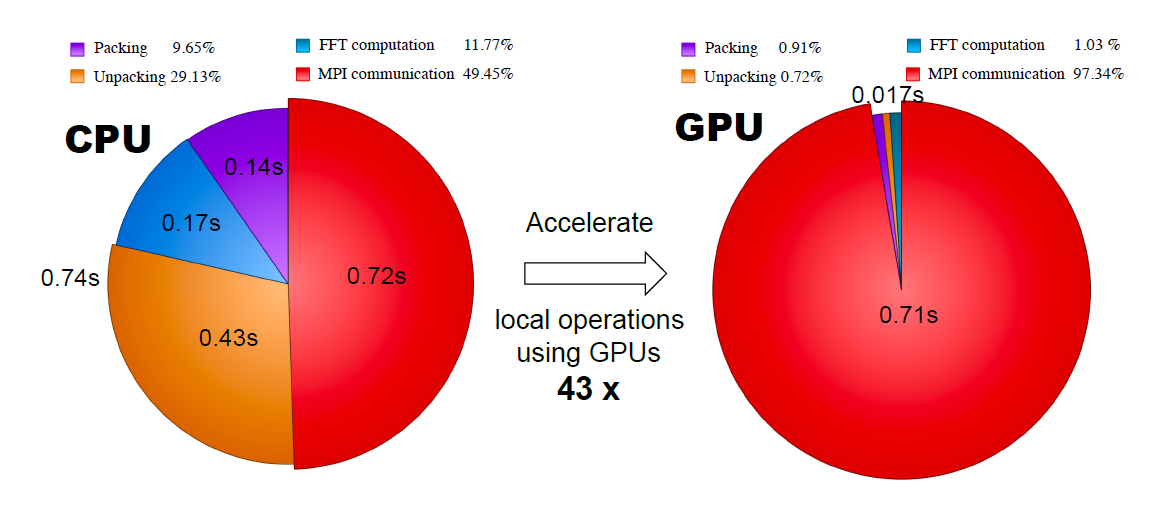
\includegraphics[width=\linewidth, keepaspectratio]{../res/speedup.png}
	\end{figure}
	\begin{itemize}
		\item $\frac{0.14s+0.17s+0.42s+0.72s}{0.017s+0.71s}=200,8\% \rightarrow$  2-fache Beschleunigung
		\item Kommunikationszeit nur vernachlässigbare Änderung
		\item rechte Seite graphisch nicht akkurat dargestellt!
	\end{itemize}
}
\frame
{
	\frametitle{Bottleneck: Kommunikation}
	Nach der Beschleunigung ist der  Zeitanteil der Kommunikation:\\
	$$\frac{0.71s}{0.71s+0.017}\approx97,6\%$$
	$\implies$ Bottleneck in der Kommunikation\\
	\large Was tun? \normalsize
}
\frame
{
	\frametitle{Was tun?}
	Konzeptionell 2 Ansätze:
	\begin{itemize}
		\item Option1: Verwendung eines besseren Algorithmus hinsichtlich serieller Anteile und Kommunikation.
		\item Option2: Verbesserung der Kommunikationsstrategie unter Einbeziehung von Eigenschaften der Systemarchitektur.
	\end{itemize}
}
\frame
{
	\frametitle{Systemarchitektur}
	\begin{figure}[h!]
		\centering
		\begin{subfigure}[t]{0.3\linewidth}
			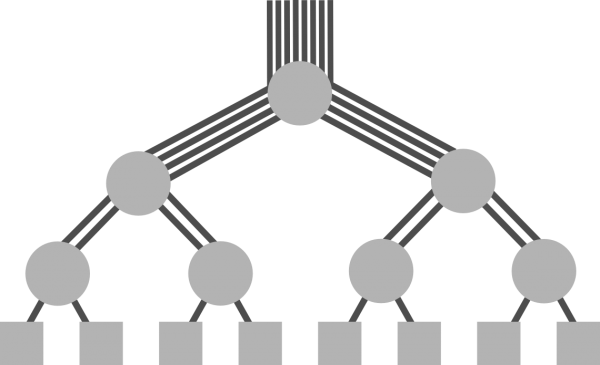
\includegraphics[width=1\linewidth]{../res/fat_tree.png}
			\footnotemark[1]
		\end{subfigure}
~
		\begin{subfigure}[t]{0.6\linewidth}
			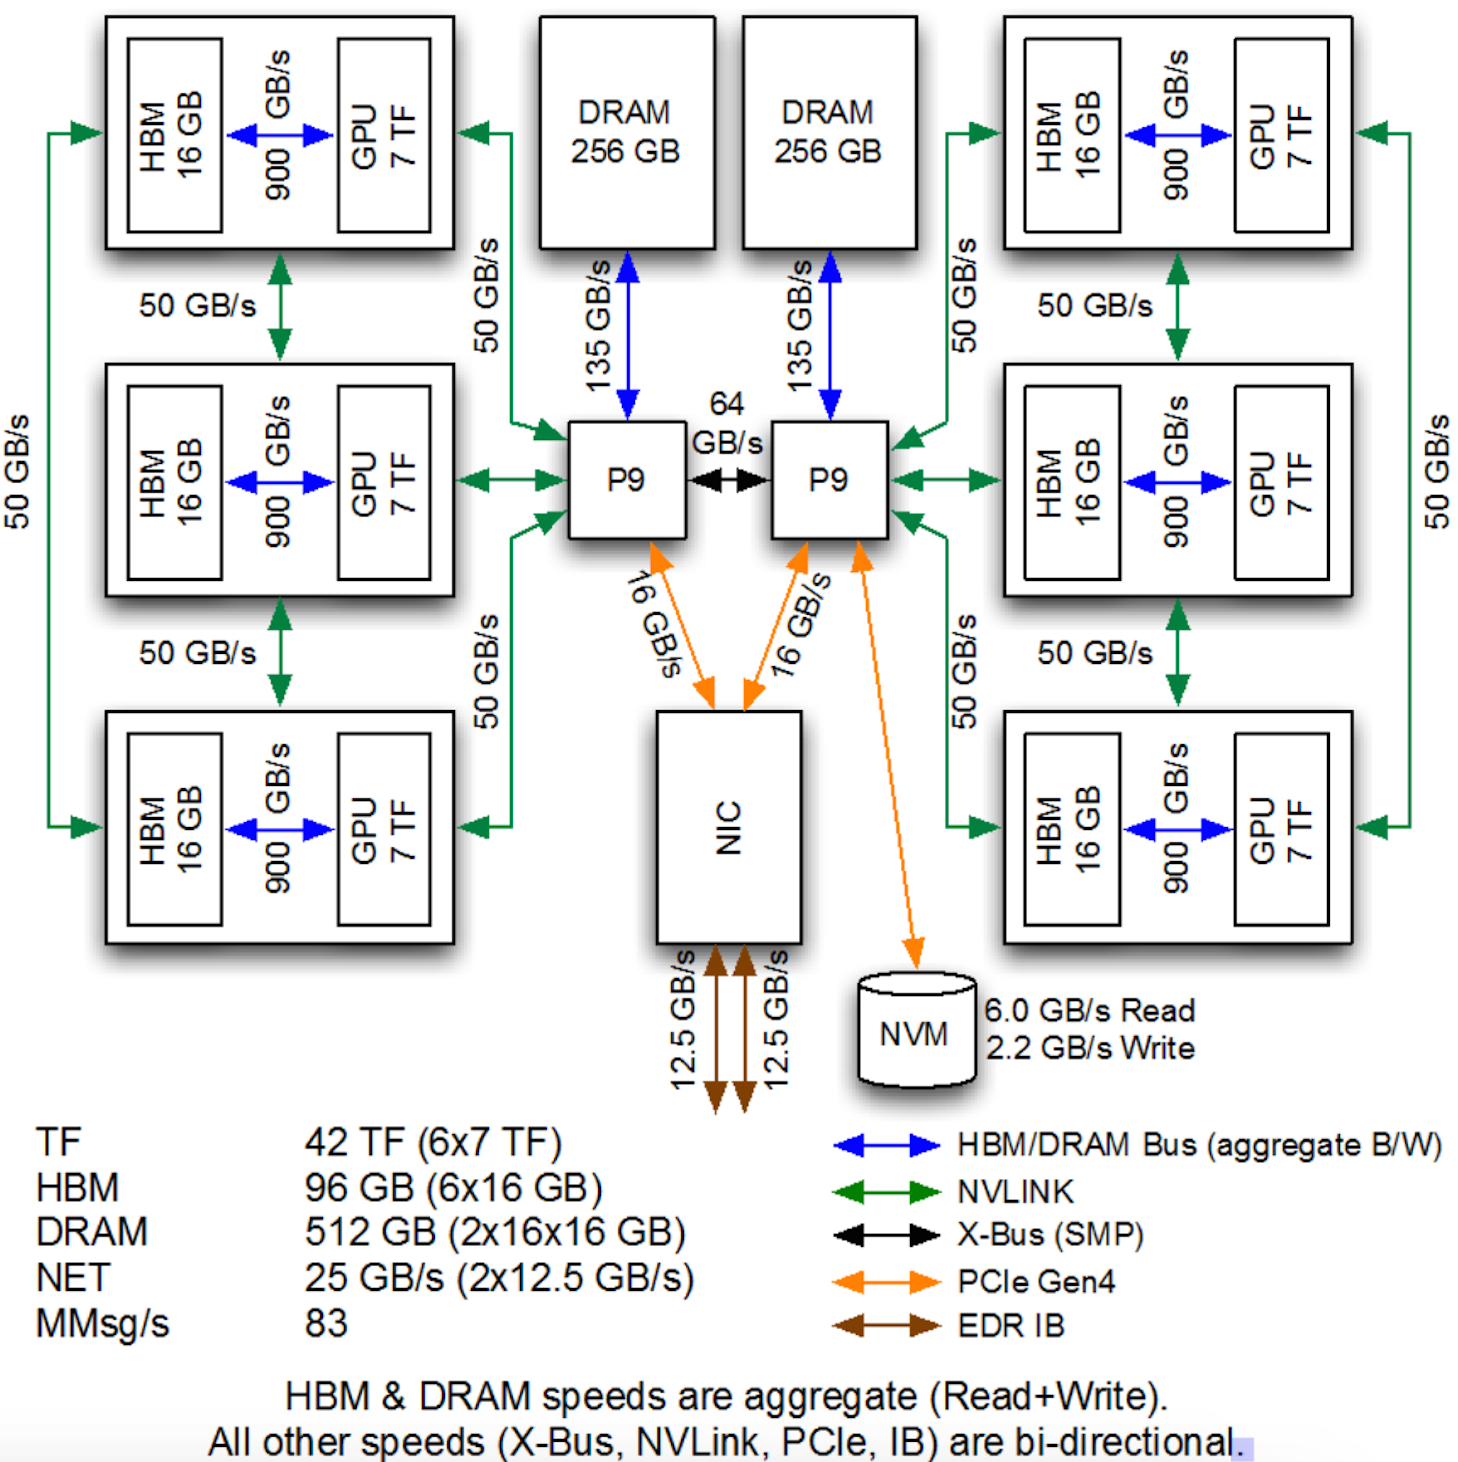
\includegraphics[width=1\linewidth]{../res/architecture.png}
			\footnotemark[2]
		\end{subfigure}
	\end{figure}

\footnotetext[1]{\tiny\url{https://clusterdesign.org/fat-trees/} am 6.2.2019\normalsize}
\footnotetext[2]{\tiny Shajek H., Tomov S., Ayala A., Haidar A., Dongarra J:\\{\sl GPUDirect MPI Communications and Optimizations to Accelerate FFTs on Exascale Systems};\\EuroMPI ’19 Posters, September 11-13, 2019, Zurich, Switzerland}
\normalsize
}
\frame
{
	\frametitle{Ansatz 0}
	Benchmarks zur Ermittlung der tatsächlichen Bandbreite.
	\begin{figure}[h!]
		\centering
		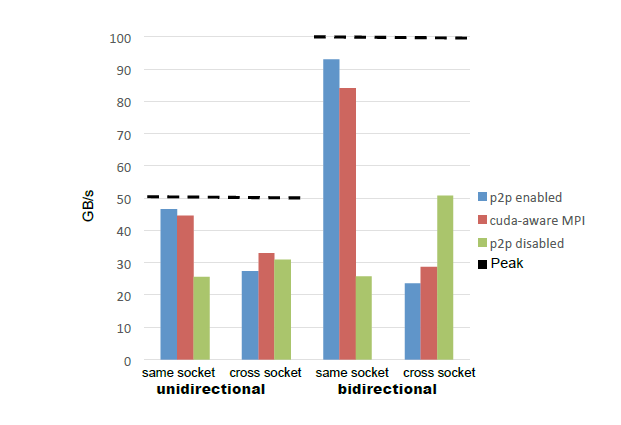
\includegraphics[width=0.7\linewidth, keepaspectratio]{../res/bench0.png}
	\footnotemark[1]
	\end{figure}
\footnotetext[1]{\tiny Shajek H., Tomov S., Ayala A., Haidar A., Dongarra J:\\{\sl GPUDirect MPI Communications and Optimizations to Accelerate FFTs on Exascale Systems};\\EuroMPI ’19 Posters, September 11-13, 2019, Zurich, Switzerland}
}
\frame
{
	\frametitle{Ansatz 1}
	Nach Option2: Untersuchung Kommunikativer Eigenschaften der Systemarchitektur
	\begin{figure}[h!]
		\centering
		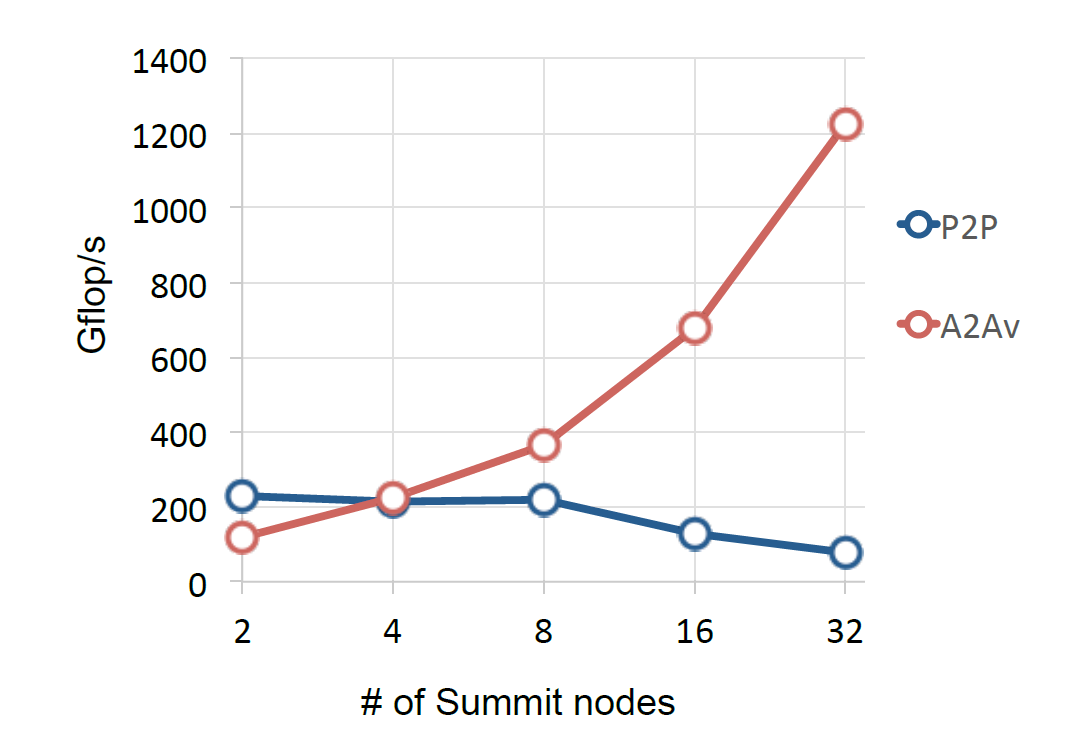
\includegraphics[width=0.7\linewidth, keepaspectratio]{../res/bench.png}
		\footnotemark[1]
	\end{figure}
\footnotetext[1]{\tiny Shajek H., Tomov S., Ayala A., Haidar A., Dongarra J:\\{\sl GPUDirect MPI Communications and Optimizations to Accelerate FFTs on Exascale Systems};\\EuroMPI ’19 Posters, September 11-13, 2019, Zurich, Switzerland}
}
\frame
{
	\frametitle{Ansatz 2}
	Nach Option1: Algorithmische Anpassung
	\begin{figure}[h!]
		\centering
		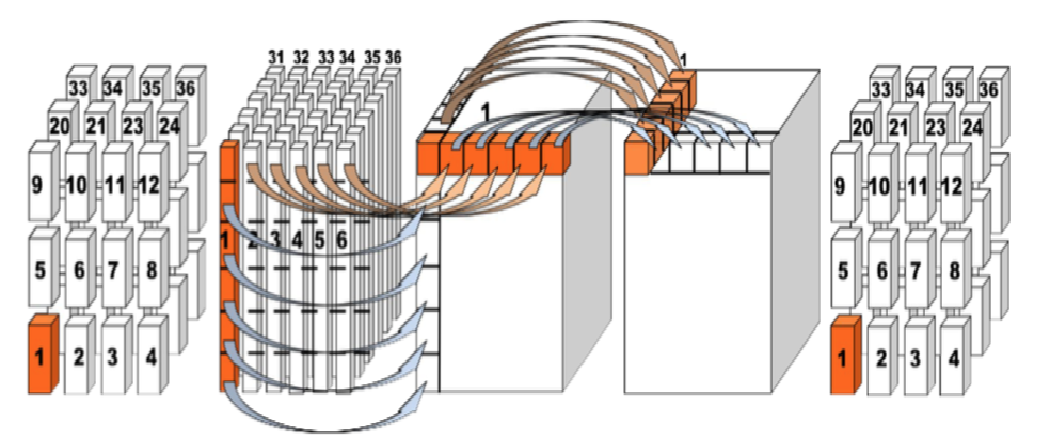
\includegraphics[width=0.7\linewidth, keepaspectratio]{../res/algo.png}
		\footnotemark[1]
	\end{figure}
	1D\textit{pencil} $\rightarrow$ 2D\textit{slabs} Übertragungsgröße
	$(TransformX,TransformY,TransformZ,MoveBack)\rightarrow(TransformY,TransformZ,MoveBack)$
	Theretisch: $25\%$ Ersparnis

\footnotetext[1]{\tiny Shajek H., Tomov S., Ayala A., Haidar A., Dongarra J:\\{\sl GPUDirect MPI Communications and Optimizations to Accelerate FFTs on Exascale Systems};\\EuroMPI ’19 Posters, September 11-13, 2019, Zurich, Switzerland}
}

\frame
{
	\frametitle{Ansatz 2}
	\begin{figure}[h!]
		\centering
		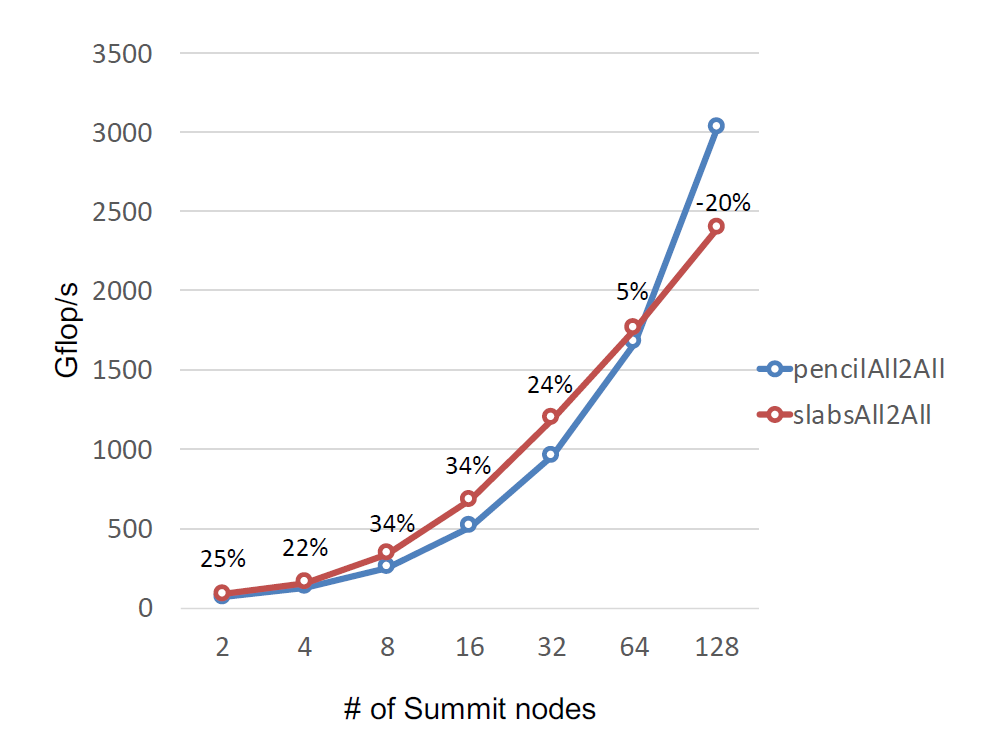
\includegraphics[width=0.7\linewidth, keepaspectratio]{../res/bench2.png}
		\footnotemark[1]
	\end{figure}
	Nachteil: Quadratischer Speicherverbrauch pro Knoten
	
\footnotetext[1]{\tiny Shajek H., Tomov S., Ayala A., Haidar A., Dongarra J:\\{\sl GPUDirect MPI Communications and Optimizations to Accelerate FFTs on Exascale Systems};\\EuroMPI ’19 Posters, September 11-13, 2019, Zurich, Switzerland}
}
\frame
{
	\frametitle{Ansatz 3}
	Dynamische Analysen hinsichtlich
	\begin{itemize}
		\item Speicherverbrauch
		\item Rechenlast
	\end{itemize}
	zur optimalen Auslastung und Aufteilung auf die Einheiten von Rechenressourcen 
	\begin{enumerate}
		\item{Knoten}
		\item{Sockel}
		\item{Prozessor}
	\end{enumerate}
	$\implies$ Vermeidung unnötiger Kommunikation.
}


%%TODO delete from here
% the following is another presentation left in for example referencing
\frame
{
	
	\frametitle{Musikklassifizierung}
	Die Einteilung von Musik innerhalb bestimmter Kategorien.
	\begin{itemize}
		\item \textbf{Genre}
		\item Mood
		\item Besetzung
		\item etc.
	\end{itemize}
$\mathbb{M}$ : Menge aller Musik \\
$\mathbb{C}$ : Menge aller Klassen einer Kategorie\\
$S$ : Menge aller bekannten Samples mit Kennzeichnung 
$$(x,y) \in S, x \in \mathbb{M}, y \in \mathbb{C}$$
$$k : \mathbb{M} \rightarrow \mathbb{C}$$
Forderung:
$$\forall (x,y) \in S : k(x) = y$$

}
\frame
{
	\frametitle{Genre}
	%TODO quote
	Durch gesellschaftliche Konventionen gebildete Einteilung in Gruppen.\\
	Beispiele im musikalischen Kontext:\\
	Rock, Pop, Rap, Hiphop, Metal, Elektro, Dubstep, Jazz, Klassik, usw.
}

\frame
{
	\frametitle{Verfügbare Daten}
	\begin{itemize}
		\item GTZAN-Datensatz\\
			10 Genres (Blues, Klassik, Country, Disco, Hiphop, Jazz, Metal, Pop, Reggae, Rock), je 100 Stücke á 30 Sekunden.
		\item OTH-Regensburg-Sammlung\\
			Laienhafte Musiksammlung, Genres Classical, Elektro, Rock Pop, Hiphop, Industrial. Nicht aufbereitet.
	\end{itemize}
	Es wurde hauptsächlich der GTZAN-Datensatz verwendet.
}

\frame
{
	\frametitle{Neuronale Netze}
	\framesubtitle{Neuronen}
	Aufgebaut aus Neuronen:
 	\begin{figure}[h!]
		\centering
		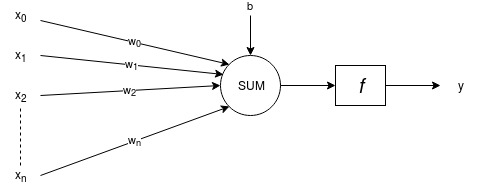
\includegraphics[width=0.8\linewidth,height=0.8\textheight, keepaspectratio]{res/old/neuron.jpg}
	\end{figure}
	$x_i$: Inputs, $y$: Output, $w_i$: Gewichte, $b$: Bias, $f$: Aktivierungsfunktion
	$$y = f((\sum_{i=0}^{n}{w_i \cdot x_i}) + b)$$
}

\frame
{	
	\frametitle{Neuronale Netze}
	\framesubtitle{Schichtenmodell}
	Angeordnet in Schichten:
 	\begin{figure}[h!]
		\centering
		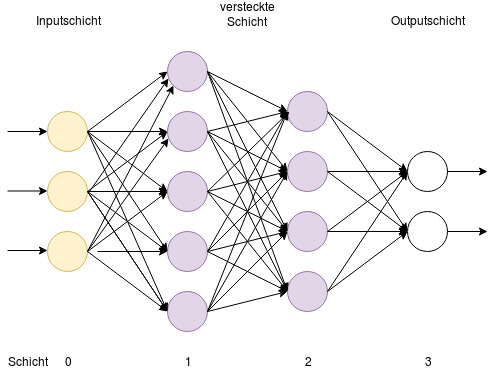
\includegraphics[width=0.8\linewidth,height=0.8\textheight, keepaspectratio]{res/old/Network.jpg}
	\end{figure}
}

\frame
{
	\frametitle{Neuronale Netze}
	\framesubtitle{Interpretation}
Ein Neuron stellt eine Abstraktion dar.\\
Neuronen/Konzepte in Folgeschichten gewichten die Relevanz von anderen Neuronen/Konzepten aus Vorgängerschichten.\\
$\Rightarrow$ Sukzessive Erhöhung des Abstraktionsgrades ist möglich.\\
Beispiel:\\
Töne $\rightarrow$ Instument $\rightarrow$ Besetzung $\rightarrow$ Genre\\
Problem bei Standardnetzen:\\
Kleine Inputvektoren gefordert, um annehmbare Modellgrößen zu gewährleisten.\\
$\Rightarrow$ u.U. viel Vorverarbeitung der Inputdaten nötig.
$\Rightarrow$ Gefahr von Informationsverlust.
}

\frame
{
	\frametitle{Deep Neural Networks}
	\framesubtitle{Motivation}
	Idee: Verwendung von Rohdaten für verlustfreien Merkmalsvektor.
	Problem: 
	\begin{itemize}
		\item Input sollte eigentlich möglichst klein sein (exponentielles Wachstum).
		\item Daten von niedrigem Abstraktionsgrad erfordern tiefe Netze.
	\end{itemize}
	Lösung: Kompensation umfangreicher Eingangsgrößen durch spezielle Schichtenarten und tiefe Netze.\\
	Beispiele: Konvolution, Rekurrenz
}

\frame
{
	\frametitle{Konvolution/Faltung}
	\begin{figure}[h!]
		\centering
		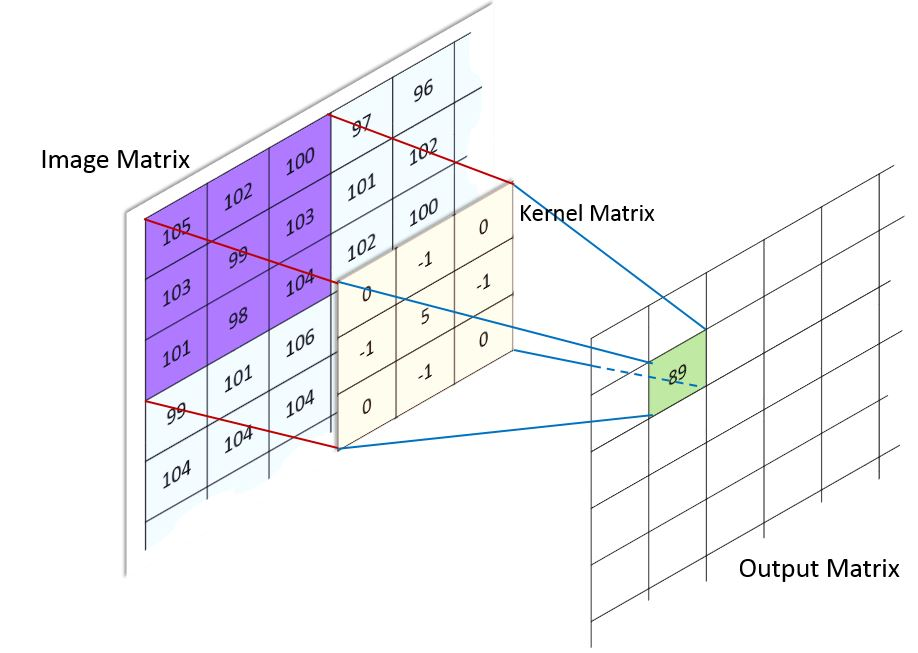
\includegraphics[width=0.7\linewidth,height=0.7\textheight, keepaspectratio]{res/old/conv.JPG}
		\footnotemark
	\end{figure}

	\footnotetext{\url{http://machinelearninguru.com/_images/topics/computer_vision/basics/convolution/1.JPG} am 13.1.2019}
}

\frame
{
	\frametitle{Rekurrenz}
	\begin{figure}[h!]
		\centering
		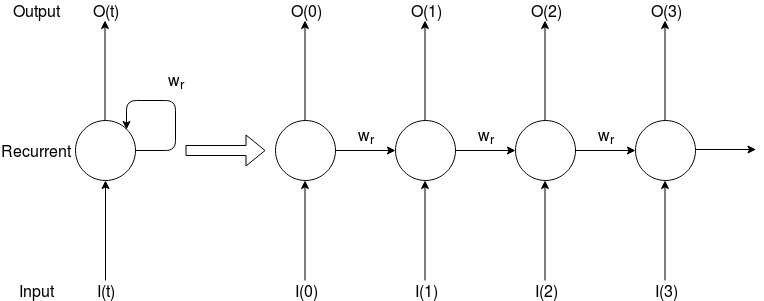
\includegraphics[width=\linewidth,height=\textheight, keepaspectratio]{res/old/recurrence.jpg}
	\end{figure}
}


\frame
{
	\frametitle{Inputformat}
	Übliche Darstellung (Amplitude-Zeit-Waveplot):
	\begin{figure}[h!]
		\centering
		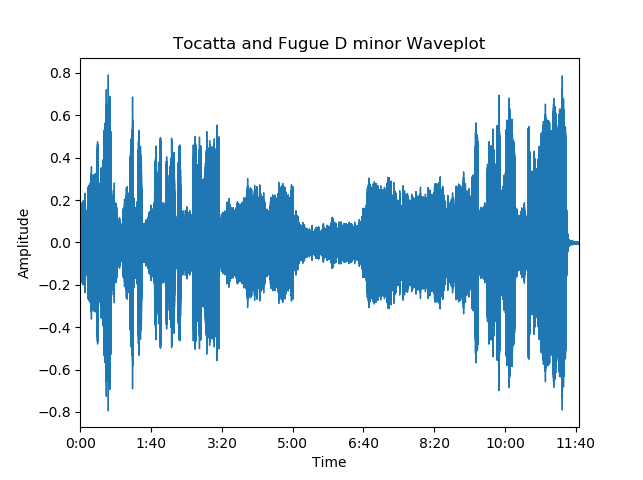
\includegraphics[width=0.8\linewidth,height=0.8\textheight, keepaspectratio]{res/old/tocattaandfuguewaveplot.png}
	\end{figure}
}

\frame
{
	\frametitle{Inputformat}
	\framesubtitle{Verbesserung}
	Kontextuell scheint Frequenzinformation wichtiger als Amplitudeninformation.\\
	Merkmale wie z.B. die Toneigenschaften eines Instruments sind über Frequenzen leichter zu erkennen.\\
	$\Rightarrow$ Fouriertransformation\\
	Um Zeitinformation zu erhalten wird die Fouriertransformation auf Zeitschlitze ausgeführt.\\
	$\Rightarrow$ Spektogramm
}

\frame
{
	\frametitle{Inputformat}
	\framesubtitle{Mel-Spektogramme}
	\begin{figure}[h!]
		\centering
		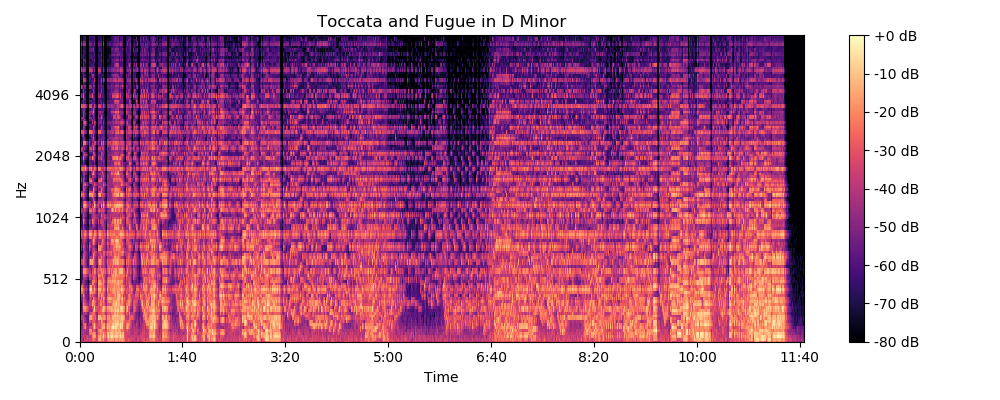
\includegraphics[width=\linewidth,height=\textheight, keepaspectratio]{res/old/tocattaandfuguemelspectogram.png}
	\end{figure}
}

\frame
{
	\frametitle{Aufbau der Netze}
	\begin{figure}[h!]
		\centering
		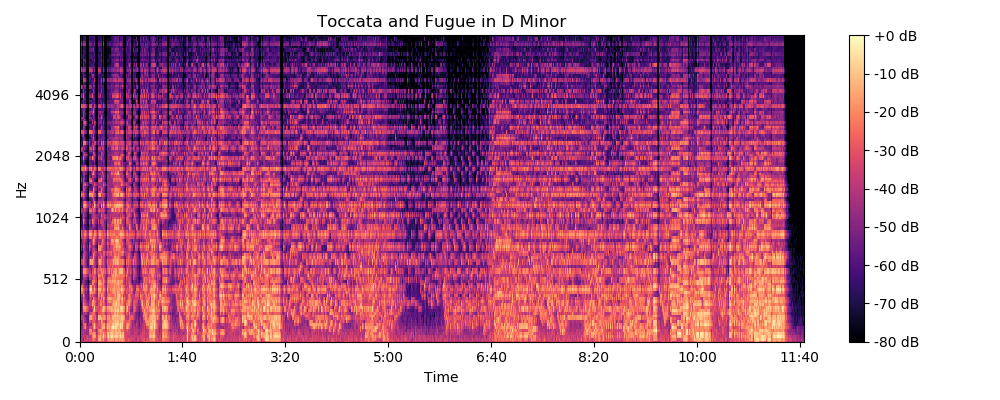
\includegraphics[width=0.7\linewidth,height=0.7\textheight, keepaspectratio]{res/old/tocattaandfuguemelspectogram.png}
	\end{figure}
	\begin{enumerate}
	\item Konvolution auf Frequenzachse.
	\item Konvolution/Rekurrenz auf Zeitachse
	\item klassische neuronale Netze zur Klassifizierung.
	\end{enumerate}
	
}

%\begin{frame}[fragile]
%\end{frame}

%\frame
%{
%	\frametitle{Datenmodell}
%	\begin{figure}[h!]
%		\centering
%		\includegraphics[width=0.9\linewidth,height=0.9\textheight, keepaspectratio]{}
%	\end{figure}
%}

\frame
{
	\frametitle{Overfitting}
	\framesubtitle{Auftreten}
	\begin{figure}[h!]
		\centering
		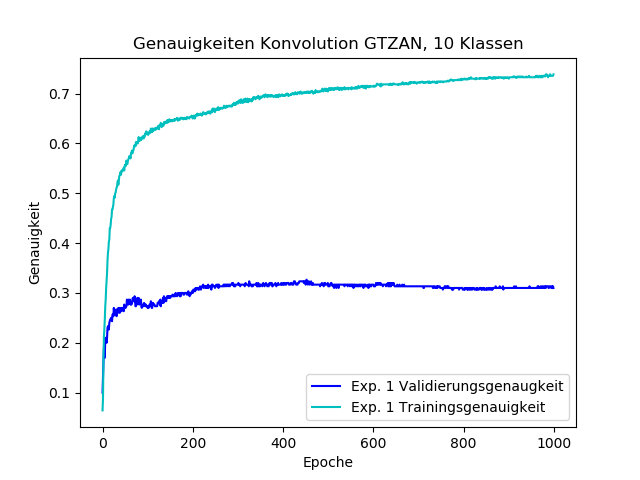
\includegraphics[width=0.7\linewidth,height=0.7\textheight, keepaspectratio]{res/old/ex1.png}
	\end{figure}
}

\frame
{
	\frametitle{Overfitting}
	\framesubtitle{Veranschaulichung}
		\begin{figure}[h!]
		\centering
		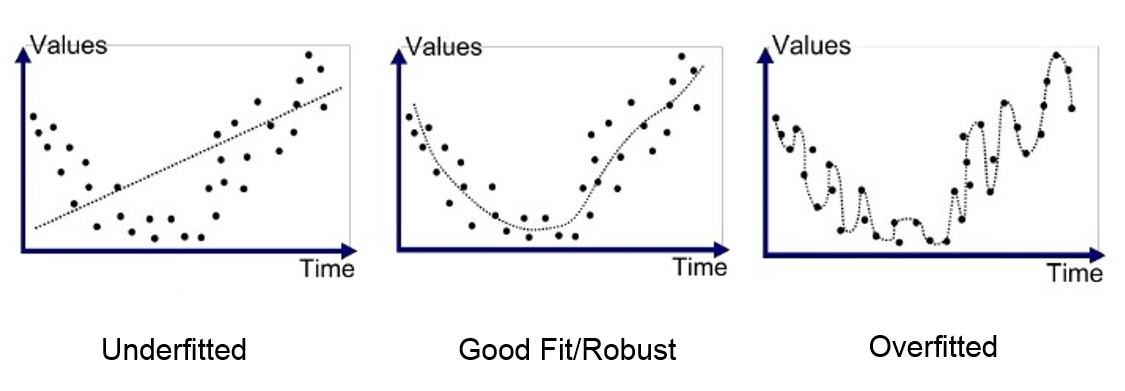
\includegraphics[width=0.9\linewidth,height=0.9\textheight, keepaspectratio]{res/old/overfitting_expl.png}
	\footnotemark
	\end{figure}

	\footnotetext{\url{https://medium.com/greyatom/what-is-underfitting-and-overfitting-in-machine-learning-and-how-to-deal-with-it-6803a989c76} am 6.2.2019}

}

\frame
{
	\frametitle{Overfitting}
	\framesubtitle{Gegenmaßnahmen}
	\begin{itemize}
		\item mehr Daten\\
			Schwer durchführbar im Rahmen der Bachelorarbeit.\\
			Realdaten sind schwierig Einzuteilen. (wenig extreme Samples, etc.)
		\item kleinere Modelle\\
	Modell muss dabei groß genug bleiben, um die Komplexität des Problems zu erfassen.\\
		(Durchgeführte Tests hierzu negativ, keine Modellgröße scheint passend)
		\item Problemverkleinerung\\
	Veringerung der Klassenanzahl. Nicht erwünscht.
	\end{itemize}
}

\frame
{
	\frametitle{Overfitting}
	\framesubtitle{Alternative Methoden}
	Datenaugmentierung: Verzerrung oder Unkenntlichmachung von irrelevanten Merkmalen in den Inputdaten.\\
	Originale, so wie Verzerrte werden zum Trainieren verwendet.\\
	Hier: Zufällig ausgewählte Zeitschlitze.
	\begin{figure}[h!]
		\centering
		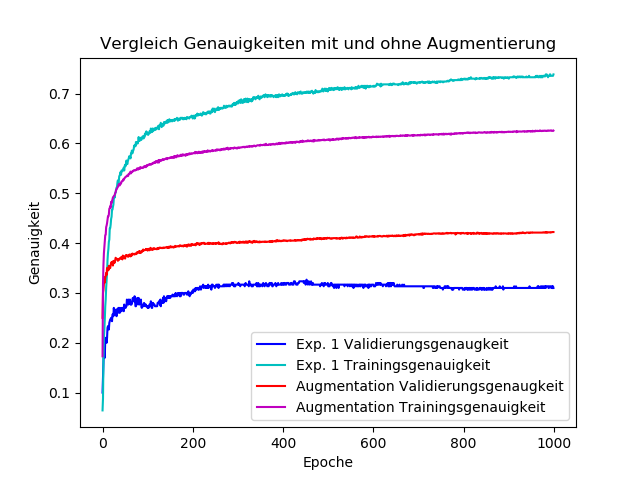
\includegraphics[width=0.5\linewidth,height=0.5\textheight, keepaspectratio]{res/old/augmentation.png}
	\end{figure}
	Die Augmentierung erschwert z.B. das Erlernen des Merkmals eines konkreten Beginns eines Stückes.
}

\frame
{
	\frametitle{Verringerung der Klassenanzahl}
	Letztendlich sind immernoch zu wenige Daten vorhanden.\\
	$\Rightarrow$ Weniger Klassen auf einmal zu klassifizieren vereinfacht das Problem.
	\begin{figure}[h!]
		\centering
		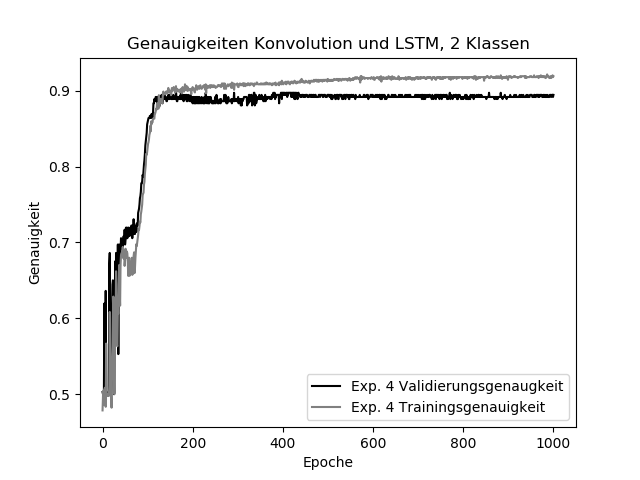
\includegraphics[width=0.5\linewidth,height=0.5\textheight, keepaspectratio]{res/old/conv_lstm.png}
	\end{figure}
	Die Kurve zeigt einen besseren Lernvorgang.
}

\frame
{
	\frametitle{Dropout}
	Zufälliger Prozentsatz der Gewichte wird auf $0$ gesetzt. (Neuronen werden abgeschaltet)\\
	$\Rightarrow$ Kompensation des übrigen Netzes.\\
	$\Rightarrow$ Langfristig stabileres Netz, dafür längere Trainingszeit
	\begin{figure}[h!]
		\centering
		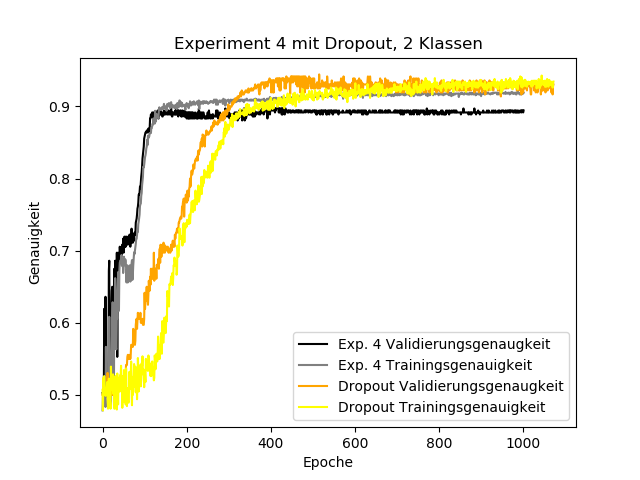
\includegraphics[width=0.5\linewidth,height=0.5\textheight, keepaspectratio]{res/old/dopout.png}
	\end{figure}
}

%\begin{frame}[fragile]
%\end{frame}

%\frame
%{
%	\frametitle{Fazit und Lehren}
%	\begin{itemize}
%	\item Aufwandsevaluation sollte vorher im Detail durchgeführt werden.
%	\item Musikalisches Fachwissen wäre äußerst Vorteilhaft.
%	\end{itemize}
%}

\frame
{
	\begin{center}
		\Large Vielen Dank für die Aufmerksamkeit!
		\normalsize
		\end{center}
}

\end{document}
